%%%%%%%%%%%%%%%%%%%%%%%%%%%%%%%%%%%%%%%%%%%%%%%%%%%%%%%%%%%%%%%
%         Estudio empírico de las funciones de activación
%%%%%%
%   1. Comparativas en cuanto a coste computacional.
%%%%%%%%%%%%%%%%%%%%%%%%%%%%%%%%%%%%%%%%%%%%%%%%%%%%%%%%%%%%%%%

\chapter{Democratización de las funciones de activación}
\label{funciones-activacion-democraticas-mas-demoscraticas}
A lo largo de este capítulo se esclarecerá la idea
que se planteó en \ref{def:funcion_activacion_articulo}
de si 
hay alguna función de activación mejor que otra. 
Para ello 
se han aportado dos nuevos resultados originales: 
el teorema \ref{teo:eficacia-funciones-activation} 
y el corolario \ref{corolario:afine-activation-function}.
Gracias a ellos se puede establecer cuándo 
dos espacios de redes neuronales con funciones de activación distintas pueden aproximar
con la misma precisión una función. Cabe mencionar 
que estos resultados son además independientes del modelo de red neuronal seleccionado gracias a los resultados teóricos descubiertos en \ref{consideration-irrelevancia-sesgo} y \ref{ch05:dominio-discreto}.

El teorema \ref{teo:eficacia-funciones-activation} 
y el corolario \ref{corolario:afine-activation-function}  tienen su importancia ya que
si sabemos que dos funciones de activación producen 
los mismos resultados, 
conociendo su coste computacional podremos seleccionar 
el que sea menor y de esta manera optimizar el tiempo 
de cálculo y disminuir el número de operaciones sin 
perder precisión en los resultados.  

Es por ello que 
tras establecer las clases de funciones que producen 
resultados similares, en la sección \ref{ch06:coste-computacional-funciones-activacion}
se ha formulado un test para
determinar las funciones de menor costo. 





\section{Caracterización de las funciones de activación}  

Por conveniencia teórica definimos las funciones de activación en \ref{def:funcion_activacion_articulo}
como una función de $\phi:\R \longrightarrow [0,1]$, no 
decreciente, con uno como límite en infinito y cero como límite a 
menos infinito; nos basaremos en el concepto \textit{actual} de función de activación:
basta con que sea una función no polinómica
(véanse  los artículos \cite{DBLP:journals/corr/SonodaM15}, \cite{modern-trainable-activation-functions} y \cite{FUNAHASHI1989183}).

Funciones no polinómicas hay infinitas y reincidimos en que a priori no hay una mejor que otra; por tanto, como criterio de selección nos guiaremos por la intuición que nos brinda la demostración del teorema \ref{teorema:2_3_uniformemente_denso_compactos}.
  La imagen de una función de activación es relevante a la hora de aproximar la función ideal desconocida, ya que reduce el número 
  de neuronas si se usa convenientemente.  
Por lo tanto, una buena heurística sería disponer de un repertorio básico de funciones de activación que contemplen distintas imágenes no polinómicas.


Además de las propuestas en \ref{def:funcion_activacion_articulo}, 
añadimos a nuestra colección las que mostramos en la tabla \ref{table:funciones-de-activation}. El criterio de selección ha sido contar con funciones de activación de formas diversas y que además sean las utilizadas de acorde (motivados por \ref{ch03:funcionamiento-intuitivo-funcion-activacion}) 

\pagebreak

\begin{table}[H] 
    \centering  
    \resizebox{\textwidth}{!}{
    \begin{tabular}{| c | c | c | c |}
        \hline
        Nombre & Expresión & Rango imagen  & Gráfica \\
        \hline
        %%%%%%%% Identidad %%%%%%%
        % Nombre: 
        %Identidad 
        %& %expresión 
        %$Id(x) = x$
        %& % Rango imagen
        %$(-\infty, +\infty)$
        %& % Gráfica
        %\begin{minipage}{\coeficienteAncho\textwidth}
        %    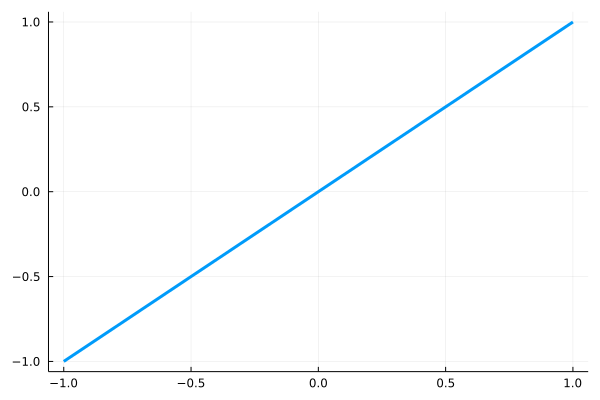
\includegraphics[width=\linewidth]{funciones-activacion/Identidad.png}
        %\end{minipage}
        %\\
        %\hline
         %%%%%%%% Indicadora %%%%%%%
        % Nombre: 
        Indicadora $\lambda \in \R$
        & %expresión 
        $Indicadora_\lambda(x) = 1_{\{x > \lambda\}}$
        & % Rango imagen
        $\{0,1\}$
        & % Gráfica
        \begin{minipage}{\coeficienteAncho\textwidth}
            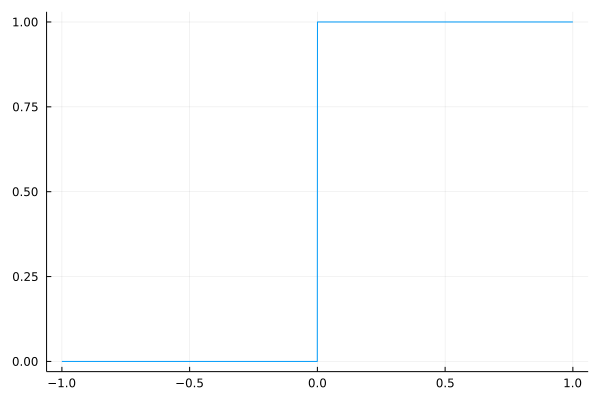
\includegraphics[width=\linewidth]{funciones-activacion/Indicadora de 0.png}
        \end{minipage}
        \\
        \hline
         %%%%%%%% Función umbral %%%%%%%
        % Nombre: 
        Función umbral $p$ polinomio
        & %expresión 
        $Umbral(x) = 1_{\{p(x) > 0\}}$
        & % Rango imagen
        $\{0,1\}$
        & % Gráfica
        \begin{minipage}{\coeficienteAncho\textwidth}
            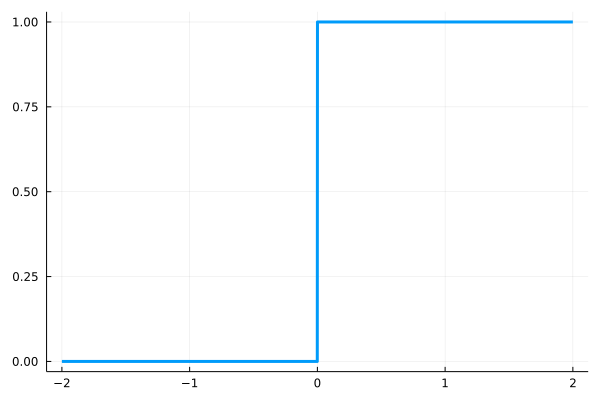
\includegraphics[width=\linewidth]{funciones-activacion/Threshold de polinomio 2x.png}
        \end{minipage}
        \\
        \hline
         %%%%%%%% Función rampa %%%%%%%
        % Nombre: 
        Función rampa
        & %expresión 
        $Rampa(x) = x 1_{\{0 < x <1\}} + 1_{\{x \geq 1\}}$ 
        & % Rango imagen
        $[0,1]$
        & % Gráfica
        \begin{minipage}{\coeficienteAncho\textwidth}
            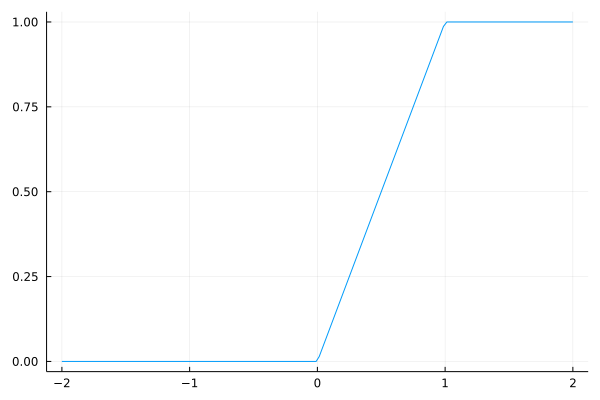
\includegraphics[width=\linewidth]{funciones-activacion/Rampa.png}
        \end{minipage}
        \\
        \hline
        %%%%%%%% sigmoide %%%%%%%%
        % Nombre: 
        Sigmoidea 
        & %expresión 
        $\sigma(x) = \frac{1}{1+e^{-x}}$
        & %Rango imagen
        $(0,1)$
        & % Gráfica
        \begin{minipage}{\coeficienteAncho\textwidth}
            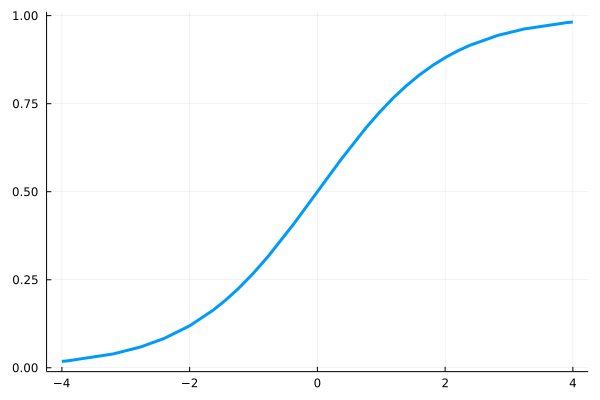
\includegraphics[width=\linewidth]{funciones-activacion/Sigmoid.png}
        \end{minipage}
        \\
        \hline
        %%%%%%%% Tangente hiperbólica  %%%%%%%%
        % Nombre: 
        Tangente hiperbólica 
        & %expresión 
        $\tanh$
        & %Rango imagen
        $(-1,1)$
        & % Gráfica
        \begin{minipage}{\coeficienteAncho\textwidth}
            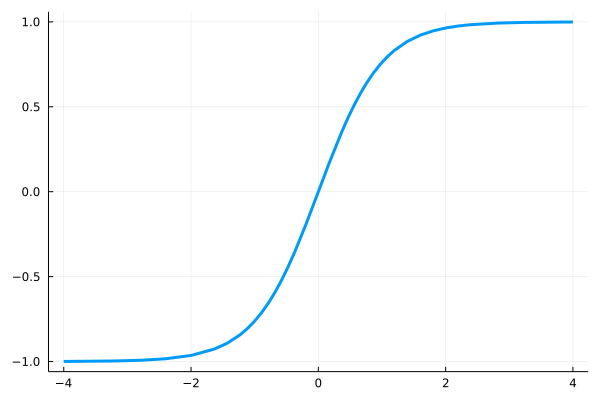
\includegraphics[width=\linewidth]{funciones-activacion/Tangente hiperbolica.png}
        \end{minipage}
        \\
        \hline
        %%%%%%%% Valor absoluto%%%%%%%%
        % Nombre: 
        Valor absoluto
        & %expresión 
        $abs(x)= |x|$
        & %Rango imagen
        $[0,+\infty]$
        & % Gráfica
        \begin{minipage}{\coeficienteAncho\textwidth}
            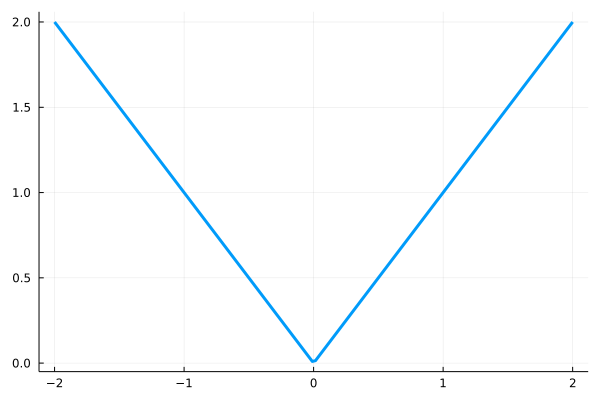
\includegraphics[width=\linewidth]{funciones-activacion/Valor absoluto.png}
        \end{minipage}
        \\
        \hline
         %%%%%%%% Coseno %%%%%%%%
        % Nombre: 
        Coseno
        & %expresión 
        $\cos$
        & %Rango imagen
        $[-1,1]$
        & % Gráfica
        \begin{minipage}{\coeficienteAncho\textwidth}
            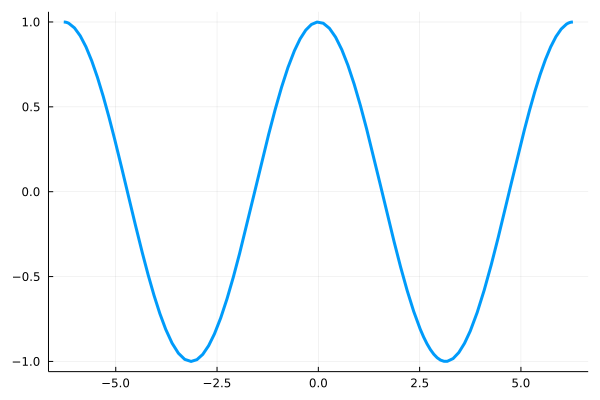
\includegraphics[width=\linewidth]{funciones-activacion/coseno.png}
        \end{minipage}
        \\
        \hline
        %%%%%%%% Cosine Squasher %%%%%%%%
        % Nombre: 
        \textit{Cosine Squasher}
        & %expresión 
        $CosineSquasher(x)=\left(1 + \cos\left(x + 3 \frac{\pi}{2} \right) \frac{1}{2}\right) 
        1_{\{\frac{-\pi}{2} \leq x \leq  \frac{\pi}{2}\}}
        +
        1_{\{ \frac{\pi}{2} < \lambda \}}.$
        & %Rango imagen
        $[0,1]$
        & % Gráfica
        \begin{minipage}{\coeficienteAncho\textwidth}
            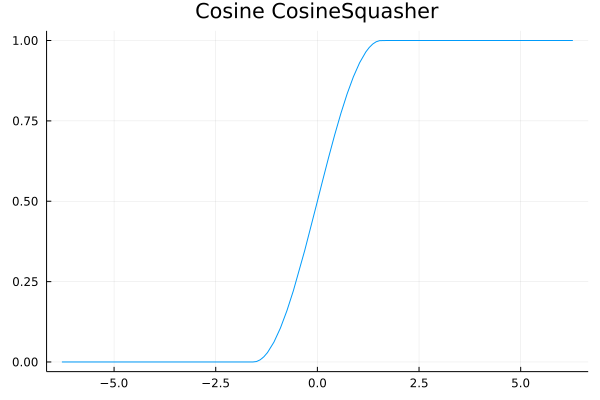
\includegraphics[width=\linewidth]{funciones-activacion/Cosine CosineSquasher.png}
        \end{minipage}
        \\
        \hline
        %%%%%%%% ReLU %%%%%%%%
        % Nombre: 
        \textit{ReLU}
        & %expresión 
        $ReLU(x) = \max(0,x)$
        & %Rango imagen
        $[0,+\infty)$
        & % Gráfica
        \begin{minipage}{\coeficienteAncho\textwidth}
            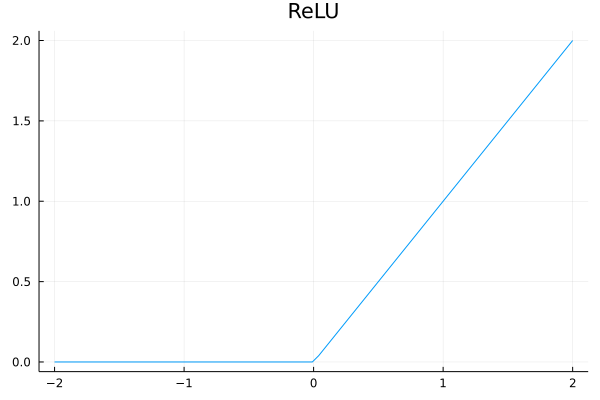
\includegraphics[width=\linewidth]{funciones-activacion/ReLU.png}
        \end{minipage}
        \\
        \hline
        %%%%%%%% Hard Hyperbolic Function %%%%%%%%
        % Nombre: 
        \textit{Hard Hyperbolic Function}
        & %expresión 
        $Hardtanh(x) =\left\{ \begin{array}{lcc}
            -1 &   si  & x \leq -1 \\
            \\ x &  si & -1< x < 1 \\
            \\ 1&  si  & x \geq 1 
            \end{array}
        \right.$
        & %Rango imagen
        $[-1,1]$
        & % Gráfica
        \begin{minipage}{\coeficienteAncho\textwidth}
            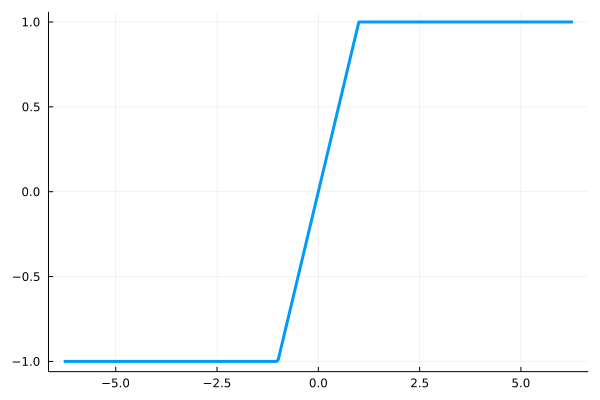
\includegraphics[width=\linewidth]{funciones-activacion/hardtanh.png}
        \end{minipage}
        \\
        \hline
        %%%%%%%% Leaky ReLU%%%%%%%
        % Nombre: 
        \textit{Leaky ReLU}
        & %expresión 
        $\begin{array}{c}

            LReLU_{\alpha}(x) =\left\{ \begin{array}{lcc}
            \alpha x &   si  & x \leq 0 \\
            \\ x&  si  & x > 0 
            \end{array}
            \right.
        \\
        \text{con } \alpha \in \R^+ \text{valor }\textit{pequeño}.
        \end{array}
        $
        & % Rango imagen
        $[0, +\infty)$
        & % Gráfica
        \begin{minipage}{\coeficienteAncho\textwidth}
            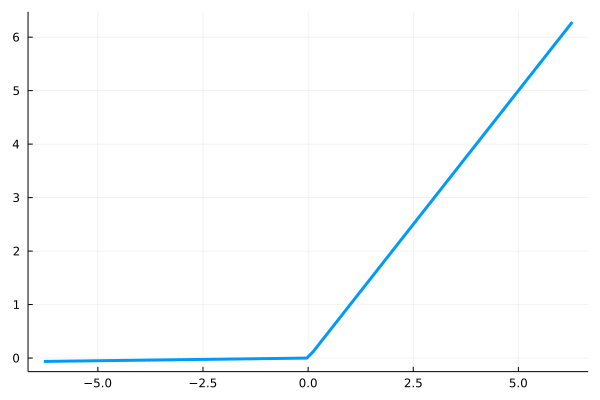
\includegraphics[width=\linewidth]{funciones-activacion/LReLU.png}
        \end{minipage}
        \\
        \hline
    \end{tabular}
    } % fin de llave de ajustarse al ancho de la página
    \caption{Compendio de funciones de activación}  
    \label{table:funciones-de-activation}
\end{table}

% comentario margen
% Qué hace la función afín definida
% y relevancia teorema 
\setlength{\marginparwidth}{\bigMarginSize}
\marginpar{\maginLetterSize
    \iconoAclaraciones \textcolor{dark_green}{     
        \textbf{
            Qué hace la función $\phi$
        }
    }

    Tal función significa aplicar traslaciones,
    simetrías, reescalados  o composiciones de estos
    movimientos a la imagen de la función afín.

    \iconoClave  \textcolor{darkRed}{     
        \textbf{
            Utilidad práctica del teorema
        }
    }

    Gracias a este resultado sabremos 
    cuándo dos funciones de activación 
    producirán exactamente los mismos resultados.
    Por lo tanto podremos seleccionar 
    la más oportuna, por ejemplo 
    la que tenga menos coste.
}


\begin{aportacionOriginal}

\begin{teorema}\label{teo:eficacia-funciones-activation}
    \label{teo:equivalencia-grafos-activation-function}
    Sea $\phi \in \mathcal{A}(\R^2)$ una función afín 
    cuya forma matricial asociada es de la forma:  
    \begin{equation}
        \phi((x,y)) =  
        \begin{bmatrix}
            a & 0 \\
             0& b 
        \end{bmatrix}
        \begin{bmatrix}
            x \\
            y
        \end{bmatrix}
        +
        \begin{bmatrix}
            t_x  & t_y
        \end{bmatrix}
    \end{equation}
    con $a,b \in \R^*$ y $t_x, t_y \in \R$.

    Sean dos funciones de activación $\sigma, \gamma$ tales que 
    \begin{equation*}
        \phi(Grafo(\sigma)) = Grafo(\gamma),
    \end{equation*}
    entonces 
    el espacio de redes neuronales de $n$ neuronas creado a partir de la función de activación $\sigma$ es  
    igual al espacio de redes neuronales creado a partir la función de activación $\gamma$. 
\end{teorema}
\begin{proof}
    % Primero lo demostramos con sesgo
    Sea $\mathcal{H}^+_{\sigma, n}(\R^d, \R^s)$ el espacio de redes neuronales con $n$ neuronas con sesgo. 

    Está claro que 
    $\mathcal{H}^+_{\gamma, n}(\R^d, \R^s)$ 
        y 
        $\mathcal{H}^+_{\sigma, n}(\R^d, \R^s)$ 
        son biyectivos.
   
    Ya que basta con tomar una red neuronal de una y cambiarle la función de activación por la de la otra. 
    Veamos 
    que se da la igualdad viendo que una está contenida en la otra. 

    Para cualquier $h  \in \mathcal{H}^+_{\sigma, n}(\R^d, \R^s)$
    la proyección i-ésima de $h$ será de la forma 

    \begin{equation*}
        h_i(x) = \sum^n_{j=1}(\beta_{j} \sigma(A_j(x))+ k_j),
    \end{equation*}
    con $x \in \R^d, \beta_{j}, k_j \in \R, A_j \in \afines$. 
    % Se define la h tilda: 
    Procedemos a definir $\tilde{h}_i(x)$ como sigue 
    \begin{align}\label{eq:h-tilda-definition}
        \tilde{h}_i(x) 
        = \sum^n_{j=1}(\beta_{j}  (b \sigma( a A_j(x) + t_x) + t_y)+ k_j)
        = \sum^n_{j=1}(\tilde{\beta}_{j} \sigma(\tilde{A}_j(x))+ \tilde{k_j}),
    \end{align}
    con $x \in \R^d, \tilde \beta_{j}, \tilde k_j \in \R, \tilde{A}_j \in \afines$,
    por lo que está claro que $\tilde{h}(x) \in \mathcal{H}^+_{\sigma, n}(\R^d, \R^s)$. 
 
    Observemos que la 
    hipótesis del enunciado 
    establece que
    \begin{align}
        Grafo(\gamma) &= \{ (x, \gamma(x)) \colon x \in \R \} 
        \\
        & = 
        Grafo(\gamma)  = \phi(Grafo(\sigma)) 
        \\
        & = 
        \phi( \{ (x, \sigma(x)) \colon x \in \R \})
        \\
        &=
        \{ (a x + t_x, b \sigma(x) + t_y) \colon x \in \R \}.
    \end{align}
    Por lo que $\tilde{h}$ así definida (\refeq{eq:h-tilda-definition})
    es a su vez 
    \begin{align}
        \tilde{h}_i(x) 
        = \sum^n_{j=1}(\beta_{j}  \gamma A_j(x)+ k_j)
    \end{align}
     es decir que $\tilde{h}(x) \in \mathcal{H}^+_{\gamma, n}(\R^d, \R^s)$. 
    Así que vía $\phi$ se ha definido una inyección 
    de $\mathcal{H}^+_{\sigma, n}(\R^d, \R^s)$ a 
    $\mathcal{H}^+_{\gamma, n}(\R^d, \R^s)$, 
    esto es 
    \begin{equation}
        \mathcal{H}^+_{\sigma, n}(\R^d, \R^s)
        \subseteq
        \mathcal{H}^+_{\gamma, n}(\R^d, \R^s).  
    \end{equation}
    Además, $\phi$ con las hipótesis exigidas es
    invertible, con inversa: 
    \begin{equation}
        \phi^{-1}((x,y)) =  
        \begin{bmatrix}
            \frac{1}{a} & 0 \\
             0& \frac{1}{b} 
        \end{bmatrix}
        \begin{bmatrix}
            x \\
            y
        \end{bmatrix}
        +
        \begin{bmatrix}
            - \frac{t_x}{a}  &  - \frac{t_y}{b}
        \end{bmatrix}.
    \end{equation}
    Así que razonando de igual manera que en el 
    apartado anterior se tiene la inclusión
    \begin{equation}
        \mathcal{H}^+_{\sigma, n}(\R^d, \R^s)
        \supseteq
        \mathcal{H}^+_{\gamma, n}(\R^d, \R^s),  
    \end{equation}
    por lo que podemos concluir que 
    \begin{equation*}
        \mathcal{H}^+_{\gamma, n}(\R^d, \R^s) 
        = 
        \mathcal{H}^+_{\sigma, n}(\R^d, \R^s).
    \end{equation*}
    Como demostramos en \ref{consideration-irrelevancia-sesgo} se tiene que 
    \begin{equation*}
        \mathcal{H}^+_{\sigma, n}(\R^d, \R^s) = \mathcal{H}^+_{\gamma, n}(\R^d, \R^s) 
        \subset 
            \mathcal{H}_{\gamma, n+1}(\R^d, \R^s) 
        \subset
        \mathcal{H}^+_{\gamma, {n+1}}(\R^d, \R^s) = \mathcal{H}^+_{\sigma, {n+1}}(\R^d, \R^s) 
        .
    \end{equation*}
    Por lo que para un $n$ arbitrariamente grande, se acaba de probar lo buscado. 
    \begin{equation*}
        \mathcal{H}_{\gamma}(\R^d, \R^s) = \mathcal{H}_{\sigma}(\R^d, \R^s).
    \end{equation*}
\end{proof}
\end{aportacionOriginal}



\subsubsection*{\iconoClave  \textcolor{darkRed}{Relevancia práctica del teorema}}
Este teorema lo que nos está diciendo es que si dos funciones de activación tienen \textit{la misma forma}
(independientemente de su grafo)
entonces \textbf{aproximarán igual de bien},
es decir, con el mismo error dentro de un conjunto de datos.
 Esto a nivel práctico  significa que \textbf{si se tienen dos funciones de activación
  \textit{con la misma forma} (\textit{o muy parecida}) elige
   la que tenga menor costo computacional}, porque a 
   nivel teórico aproximarán igual de bien y de esta
    manera ahorraremos recursos. 

Notemos además que la demostración nos enseña que la igualdad se da independientemente del número de 
neuronas fijado, es decir que no es un resultado 
asintótico (lo asintótico en términos prácticos 
significa que sea resultado de una serie de 
aproximaciones).  

% Relevancia corolario 
\marginpar{\maginLetterSize
    \iconoAclaraciones \textcolor{dark_green}{     
        \textbf{
            Relevancia corolario 
            \ref{corolario:afine-activation-function}
        }
    }
    Simplifica las comparativas entre funciones 
    de activación 
    sin necesidad de conocer su imagen.
}
%corolario para cuando sean afines 
\begin{corolario}\label{corolario:afine-activation-function}
    Sea $\phi \in \mathcal{A}(\R)$ una transformación afín e invertible, esto es de la forma 
    \begin{equation}
        \phi(x) = a x + b 
        \text{ con } a \in \R^*, b \in \R.
    \end{equation}
    Dadas dos funciones de activación $\sigma$ y $\gamma$ que satisfagan que 
    \begin{equation}
        \phi \circ \sigma = \gamma,
    \end{equation} 
    entonces 
    el espacio de redes neuronales de $n$ neuronas creado con la función de activación $\sigma$ es  
    igual al espacio de redes neuronales creado con la función de activación $\gamma$. 
\end{corolario}
\begin{proof}
    En base a que $\phi(x) = a x + b$, con 
    $a \in \R^*, b \in \R$
    basta con definir 
     $\psi  \in \mathcal{A}(\R^2)$ como 
    \begin{equation}
        \psi((x,y)) =  
        \begin{bmatrix}
            1 & 0 \\
             0& a
        \end{bmatrix}
        \begin{bmatrix}
            x \\
            y
        \end{bmatrix}
        +
        \begin{bmatrix}
            0 & b
        \end{bmatrix}.
    \end{equation}
    A partir  definición se tiene que 
    \begin{align}
        Grafo(\gamma) &=
        \{ (x, \gamma(x)) \colon x \in \R\} 
        \\
        & = 
        \{ (x, \phi(\sigma(x))) \colon x \in \R\}
        \\
        & =
        \psi(\{ (x, \sigma(x)) \colon x \in \R\})
        = 
        \psi(Grafo(\sigma)).
    \end{align}
    Se satisfacen 
    las hipótesis del teorema \ref{teo:equivalencia-grafos-activation-function} y en virtud de él se tiene el resultado buscado.
\end{proof}

\section{ Selección de las mejores funciones de activación}
Así pues, a la vista de la imágenes de las distintas funciones de activación 
recogidas en la tabla \ref{table:funciones-de-activation}, y
por el recién probado teorema \ref{teo:eficacia-funciones-activation}, podemos determinar a priori 
que de manera teórica existen conjuntos de funciones que aproximadamente  pueden producir los mismos resultados. 

A la vista de del resultado, si las funciones de 
activación son similares entonces actuarán con 
una precisión similar, es por ello 
que el la table \ref{table:Clases-equivalencia-activation-function} establecemos 
las siguientes clases de funciones de activación 

\begin{table}[H] 
    \centering  
    \begin{tabular}{| c | c | c | }
        \hline
        \textit{Grupo escalera} & \textit{Grupo sigmoide} & \textit{Grupo ReLU} \\
        \hline
       &  Rampa &  \\
       Indicadora & Sigmoidea & ReLU\\
       Umbral & \textit{Cosine Squasher}& LReLU\\
        & tanh & \\
        & \textit{Hard Hyperbolic Function}& \\
\hline
    \end{tabular}
    \caption{Agrupaciones de funciones de activación con forma similar}  
    \label{table:Clases-equivalencia-activation-function}
\end{table}

Compararemos entonces su coste computacional y tomaremos como representante de la clase aquel que sea de menor coste. 


% Comentario aclaratorio de qué es indirección 
\setlength{\marginparwidth}{\bigMarginSize}
\marginpar{\maginLetterSize
    \iconoAclaraciones \textcolor{dark_green}{     
        \textbf{
            Significado indirección 
        }
    }

    La indirección es una técnica de programación 
    que consiste en hacer una referencia indirecta 
    a los datos usando direcciones en memoria. 
    Esto conlleva el almacenamiento en memoria no solo 
    de los datos, si no de las direcciones (que no deja de ser un dato más).   
}

% Comentario aclaratorio de qué es indirección 
\marginpar{\maginLetterSize
    \iconoAclaraciones \textcolor{dark_green}{     
        \textbf{
            Significado \textit{overhead}
        }
    }

    Hace referencia a el coste  computacional adicional 
    que conllevan resolver las indirecciones en este caso.
}


\subsection{ Implementación de las funciones de activación en la biblioteca de redes neuronales} 
\label{ch06:activation-function-implementation}
Las funciones de activación han sido implementadas con cuidado de que sean eficientes 
y valiéndose de las características propias de Julia, para ello se han utilizado técnicas como: 

\begin{itemize}
    % Programación modular 
    \item \textbf{Programación modular}: Tal y como se recomienda en la documentación de Julia \footnote{
        Consultada en la página web oficial de Julia  a día 23 de mayo del 2022 con URL: \url{https://docs.julialang.org/en/v1/manual/modules/}
    } se ha utilizado un módulo en la implementación de la biblioteca, esto aporta los siguientes beneficios: 
    \begin{itemize}
        \item Los módulos pueden ser precompilados y de esta manera se aceleraría la carga y el tiempo de inicialización. 
        \item Encapsulamiento de los métodos y facilidades de uso del espacio de nombres, lo cual forma parte
        de una buena metodología de programación. 
    \end{itemize}

    % Macros
    \item \textbf{Macros}\footnote{La información consultada de macros ha sido  de la página oficial de Julia, a día 23 de mayo del 2022, URL:
    \url{https://docs.julialang.org/en/v1/manual/metaprogramming}}:
    que permiten sustituciones de código cuando éste es analizado por el compilador; 
    de esta manera, funciones que devuelven otras funciones dependientes de un parámetro se verán beneficiadas,
    ya que hace que se ejecute código más rápido evitando indirecciones \footnote{La fuente bibliográfica ha sido la \href{https://es.wikipedia.org/wiki/Indirección}{Wikipedia}, a día 26 de mayo del 2022.
    También recomendamos especialmente la entrada en inglés de la misma:
    \href{https://en.wikipedia.org/wiki/Indirection}{\textit{Indirection}}
    consultada también el día 26 de mayo del 2022.
    }  y el overhead correspondiente. 
     Puede encontrar la implementación de esto en la biblioteca de redes neuronales implementada en nuestro 
     repositorio 
     \footnote{
         Esto es en \url{https://github.com/BlancaCC/TFG-Estudio-de-las-redes-neuronales/tree/main/OptimizedNeuralNetwork.jl/src/activation_functions.jl}
     }.

     % Funtores 
     \item Funtores o como son llamados en Julia \href{https://docs.julialang.org/en/v1/manual/methods/#Function-like-objects}{\textit{Function-like objects}}. Junto con las macros son una forma eficiente definir funciones de funciones y valores por defecto. 
\end{itemize}

Además la implementación de la biblioteca se ha hecho de acorde 
al \textbf{principio de sustitución de Liskov} (publicado en el artículo \cite{Liskov-principle}) que dice así: 

\enquote{
    Sea $\phi(x)$ una propiedad comprobable acerca de los objetos $x$ de tipo $T$. 
    Entonces $\phi(y)$  debe ser verdad para los objetos $y$ del tipo $S$, donde $S$ es un 
    subtipo de $T$. 
}

Esto significa que todas deben de comportarse
como una función de activación abstracta y poder intercambiarse entre ellas. 
Lo que en un principio suena obvio, ha supuesto un diseño cuidadoso y un uso de las herramientas que brinda Julia en toda 
su plenitud, puesto que tengamos en cuenta que la variabilidad a la hora de definir y caracterizar a una función de activación, ya que algunas no dependen de ningún parámetro 
mientras que otras lo hacen incluso de otras funciones (ver definiciones en la tabla \ref{table:funciones-de-activation}). 

% Nota sobre porqué nos interesa ajustar el dominio
\reversemarginpar
\setlength{\marginparwidth}{\smallMarginSize}
\marginpar{\maginLetterSize
\iconoClave \textcolor{darkRed}{     
    \textbf{
        Interés de controlar el dominio de una función
    }
} 

Lo cual permitiría optimizar la evaluación de la función; 
ya que si la función tuviera comportamientos diferentes en función del rango, 
habría que estudiarlos con condiciones interiores que aumentan el costo computacional.
}
\setlength{\marginparwidth}{\bigMarginSize}
\normalmarginpar 
% fin de la nota, comienza explicación 

% Nota en margen sobre tipos estáticos y dinámicos 
\marginpar{\maginLetterSize
\iconoAclaraciones \textcolor{dark_green}{     
    \textbf{
        Tipos estáticos y dinámicos
    }
}

    El tipo de dato \textbf{estático} se define en memoria 
    antes de la ejecución del código (durante la compilación del código),
    no pudiendo cambiar 
    durante la ejecución del programa. 
    
    Un tipo de dato \textbf{dinámico} puede cambiar y el tipo es determinado mediante 
    la ejecución. 

    Por lo general las ventajas del estático son mayor eficiencia y prevención de errores,
    por el contrario, tipos dinámicos permiten más flexibilidad a la hora de diseñar 
    y escribir el código. 
}
% Nota en margen sobre tipos nominal 
\marginpar{\maginLetterSize
\iconoAclaraciones \textcolor{dark_green}{     
    \textbf{
        Tipo de dato nominal
    }
}
Dos tipos de datos diferentes serán equivalentes o compatibles, 
si y solo si se ha hecho de manera explícita. 
Por ejemplo si definiéramos un tipo de datos de número real y otro de número 
racional, solo podríamos sumarlos si le explicáramos al ordenador cómo hacerlo. 
}
 % Nota en margen sobre tipos paramétricos 
 \marginpar{\maginLetterSize
 \iconoAclaraciones \textcolor{dark_green}{     
     \textbf{
         Tipos de datos paramétricos 
     }
 }
 Hace referencia al polimorfismo paramétrico, 
 esto es que una misma función se puede programar 
 para que actúe en consecuencia al tipo de datos que recibe 
 como argumento. 
 }
%Fin de la nota
 
% Sistema de tipos
\subsubsection*{Sobre el sistema de tipos de Julia}
\label{ch06:sistema-timpos-julia}
    Julia posee un sistema de tipos muy rico 
    \footnote{
        Véase la documentación oficial de Julia sobre \textit{Types}: 
        \url{https://docs.julialang.org/en/v1/manual/types/}. 
        Esta URL fue consultada el 26 de mayo de 2022.
    }
    dinámico, nominal y paramétrico; pero que ofrece la posibilidad de obtener
    beneficio de los tipos estáticos.
    Podría entonces uno plantearse 
    sacar provecho de esto en la \textcolor{darkRed}{declaración 
    del dominio} e imagen de una función de activación y prevención de errores. 
 
    
    Ante esta situación hemos determinado que el tipo más conveniente a usar en nuestras 
    implementaciones es el racional no sólo por
    por la observación que comentábamos en la nota marginal del teorema 
    \ref{teo:densidad-racional}
    ; ya que como
    procedemos a explicar un tipo más restrictivo
    plantea los siguientes problemas:  

     \begin{itemize}
         \item Los datos se conocen en tiempo real, luego no es posible discriminar su tipo en tiempo de compilación. La única hipótesis que tenemos de los mismos es que son racionales.  
         
         \item En caso de determinar su tipo en tiempo real estaríamos trasladando la 
         condición de rango que queríamos evitar
         a otro lugar de la implementación, 
         por lo tanto seguiría existiendo tal coste. 
         
        \item En nuestra implementación concreta solo beneficiaría a la función de activación \textit{HardTanh} y su implementación no sería satisfactoria porque no habría forma de implementar eficientemente el rango. Ejemplificamos lo que se quiere decir en el código que mostramos a continuación: 
        \begin{itemize}
            \item Entre las líneas 1 y 9 puede verse cómo definir un tipo de dato dominio en Julia.
            \item Entre las líneas 11-13 y las 16-18 cómo se declaran funciones en dominios concretos. 
            \item La línea 14 daría error, la hemos dejado para mostrar que no es posible una declaración de rangos que cumpla el principio de sustitución de Liskov y adapte eficientemente los rangos indicados.
        \end{itemize}
         
     \end{itemize}

     \begin{minipage}{\textwidth}%
     \begin{minted}
        [
        frame=lines,
        %framesep=2mm,
       % baselinestretch=1.2,
        %bgcolor=sutilGreen, 
        linenos
        ]{Julia}
        struct IntervaloCentral{T<:Real} <: Real
        x::T
        function IntervaloCentral{T}(x::T) where T<:Real
            if(-1 > x || x > 1)
                error("No está en intervalo")
            end
            new(x)
        end
    end
    
     function HardTanh(x::IntervaloCentral)
        x.x
    end
    HardTanh(x::Real)=HardTanh(convert(::IntervaloCentral,x))
    
     function HardTanh(x::Real)::Int
        sign(x)
    end
     \end{minted}
\end{minipage} 

\subsection*{Sobre la implementación definitiva y ejemplo de uso}
Puede encontrar la implementación definitiva de las funciones de activación en 
el directorio y fichero \texttt{OptimizedNeuralNetwork.jl/src/activation\_function.jl} de nuestro repositorio. 
Además en \href{https://github.com/BlancaCC/TFG-Estudio-de-las-redes-neuronales/blob/main/Memoria/capitulos/Ejemplo-uso-biblioteca.ipynb}{
    directorio y fichero \texttt{Memoria/capitulos/Ejemplo-uso-biblioteca.ipynb}}
encontrará un 
\textit{Jupyter notebook} de Julia con ejemplos de cómo llamar y utilizar las funciones de activación. 


\subsection{Coste computacional funciones activación }
\label{ch06:coste-computacional-funciones-activacion}

\subsubsection{Diseño del experimento}
El experimento para comparar los resultados ha consistido en: 
Se ha evaluado cada función a comparar $20.000.000$ veces y se ha medido cuanto tarda. 
Esto se ha repetido $15$ veces. Puede encontrar la implementación concreta y los resultados concretos de cada iteración en el repositorio del
proyecto \footnote{En el directorio de experimentos 
de \url{https://github.com/BlancaCC/TFG-Estudio-de-las-redes-neuronales}.}.
Además, puesto que las funciones más simples que se pueden construir son la identidad y la constante, las hemos añadido para poder comparar el costo. 

\subsubsection{Test de hipótesis}

Compararemos si los resultados son significativos utilizando la \textbf{prueba de los rangos con 
signo de Wilcoxon} (véase \cite{OpenIntroStatistics}, \cite{BiologicalStatistics}, o la web de \href{https://www.cienciadedatos.net}{cienciadedatos.net} \footnote{
 Prueba de los rangos con signo de Wilcoxon by Joaquín Amat Rodrigo, available under a Attribution 4.0 International (CC BY 4.0) at
  \url{https://www.cienciadedatos.net/documentos/18_prueba_de_los_rangos_con_signo_de_wilcoxon}
  Con fecha de visita el 22 de mayo del 2022.
  }).

  La motivación de realizar esta prueba es la siguiente: 
\begin{itemize}
    \item Las muestras son independientes.
    \item Los datos tomados permiten ser ordenados. 
    \item El tamaño de muestra es pequeño y no podemos asegurar normalidad de la datos. 
\end{itemize}

\subsubsection*{Hipótesis} 

\begin{itemize}
    \item $H_0$: La mediana de las diferencias de cada par de datos es $0$. 
    \item $H_a$: La mediana de las diferencias entre cada par de datos es diferente de cero. 
\end{itemize}

La utilidad de este test es que si rechaza la hipótesis nula sabremos que con un $95 \%$ de certeza tendrán medianas diferentes, es decir, \textbf{existe una 
diferencia de tiempos}. En caso de que no se rechace no podremos afirmar nada.
Puede encontrar la implementación en el repositorio del
 proyecto \footnote{En el directorio de experimentos 
 de \url{https://github.com/BlancaCC/TFG-Estudio-de-las-redes-neuronales}.}.

 Los resultados del test de Wilcoxon han sido los siguientes: 

 \begin{table}[H]
    \resizebox{\textwidth}{!}{
    \begin{tabular}{|l|l|l|l|l|l|}
    \hline
        ~ & cte 1  & Identidad  & Umbral de $2x$ & CosineSquasher & Indicadora de 0 \\ \hline
        cte 1  & - &\textbf{No rechaza $H_0$} & Rechaza $H_0$ & Rechaza $H_0$ & Rechaza $H_0$ \\ \hline
        Identidad  & \textbf{No rechaza $H_0$} & - & Rechaza $H_0$ & Rechaza $H_0$ & Rechaza $H_0$ \\ \hline
        Umbral de $2x$ & Rechaza $H_0$ & Rechaza $H_0$ & - & Rechaza $H_0$ & \textbf{No rechaza $H_0$} \\ \hline
        CosineSquasher & Rechaza $H_0$ & Rechaza $H_0$ & Rechaza $H_0$ & - & Rechaza $H_0$ \\ \hline
        Indicadora de 0 & Rechaza $H_0$ & Rechaza $H_0$ & \textbf{No rechaza $H_0$} & Rechaza $H_0$ & - \\ \hline
        Rampa & Rechaza $H_0$ & Rechaza $H_0$ & \textbf{No rechaza $H_0$} & Rechaza $H_0$ & Rechaza $H_0$ \\ \hline
        ReLU & Rechaza $H_0$ & Rechaza $H_0$ & \textbf{No rechaza $H_0$} & Rechaza $H_0$ & \textbf{No rechaza $H_0$} \\ \hline
        Sigmoidea& Rechaza $H_0$ & Rechaza $H_0$ & Rechaza $H_0$ & Rechaza $H_0$ & Rechaza $H_0$ \\ \hline
        Tangente hiperbólica & Rechaza $H_0$ & Rechaza $H_0$ & Rechaza $H_0$ & Rechaza $H_0$ & Rechaza $H_0$ \\ \hline
        Valor absoluto & Rechaza $H_0$ & Rechaza $H_0$ & Rechaza $H_0$ & Rechaza $H_0$ & Rechaza $H_0$ \\ \hline
        Coseno & Rechaza $H_0$ & Rechaza $H_0$ & Rechaza $H_0$ & Rechaza $H_0$ & Rechaza $H_0$ \\ \hline
        Hardtanh & Rechaza $H_0$ & Rechaza $H_0$ & Rechaza $H_0$ & Rechaza $H_0$ & Rechaza $H_0$ \\ \hline
        LReLU & Rechaza $H_0$ & Rechaza $H_0$ & \textbf{No rechaza $H_0$} & Rechaza $H_0$ & \textbf{No rechaza $H_0$} \\ \hline
    \end{tabular}
    }
    \caption{Resultados 1 de 3: Rechazos con un $95\%$ de confianza en el test Wilcoxon.}
    \label{Rechazo-1-de-3}
\end{table}

\begin{table}[H]
    \resizebox{\textwidth}{!}{
    \begin{tabular}{|l|l|l|l|l|}
    \hline
        ~ & Rampa & ReLU & Sigmoidea& Tangente hiperbólica \\ \hline
        cte 1  & Rechaza $H_0$ & Rechaza $H_0$ & Rechaza $H_0$ & Rechaza $H_0$ \\ \hline
        Identidad  & Rechaza $H_0$ & Rechaza $H_0$ & Rechaza $H_0$ & Rechaza $H_0$ \\ \hline
        Umbral de $2x$ & \textbf{No rechaza $H_0$} & \textbf{No rechaza $H_0$} & Rechaza $H_0$ & Rechaza $H_0$ \\ \hline
        CosineSquasher & Rechaza $H_0$ & Rechaza $H_0$ & Rechaza $H_0$ & Rechaza $H_0$ \\ \hline
        Indicadora de 0 & Rechaza $H_0$ & \textbf{No rechaza $H_0$} & Rechaza $H_0$ & Rechaza $H_0$ \\ \hline
        Rampa & - & \textbf{No rechaza $H_0$} & Rechaza $H_0$ & Rechaza $H_0$ \\ \hline
        ReLU & \textbf{No rechaza $H_0$} & - & Rechaza $H_0$ & Rechaza $H_0$ \\ \hline
        Sigmoidea& Rechaza $H_0$ & Rechaza $H_0$ & - & Rechaza $H_0$ \\ \hline
        Tangente hiperbólica & Rechaza $H_0$ & Rechaza $H_0$ & Rechaza $H_0$ & - \\ \hline
        Valor absoluto & Rechaza $H_0$ & Rechaza $H_0$ & Rechaza $H_0$ & Rechaza $H_0$ \\ \hline
        Coseno & Rechaza $H_0$ & Rechaza $H_0$ & Rechaza $H_0$ & Rechaza $H_0$ \\ \hline
        Hardtanh & Rechaza $H_0$ & Rechaza $H_0$ & Rechaza $H_0$ & Rechaza $H_0$ \\ \hline
        LReLU & \textbf{No rechaza $H_0$} & \textbf{No rechaza $H_0$} & Rechaza $H_0$ & Rechaza $H_0$ \\ \hline
    \end{tabular}
    }
    \caption{Resultados 2 de 3: Rechazos con un $95\%$ de confianza en el test Wilcoxon.}
    \label{Rechazo-2-de-3}
\end{table}

\begin{table}[H]
    \resizebox{\textwidth}{!}{
    \begin{tabular}{|l|l|l|l|l|}
    \hline
        ~ & Valor absoluto & Coseno & Hardtanh & LReLU \\ \hline
        cte 1  & Rechaza $H_0$ & Rechaza $H_0$ & Rechaza $H_0$ & Rechaza $H_0$ \\ \hline
        Identidad  & Rechaza $H_0$ & Rechaza $H_0$ & Rechaza $H_0$& Rechaza $H_0$ \\ \hline
        Umbral de $2x$ & Rechaza $H_0$ & Rechaza $H_0$ & Rechaza $H_0$ & \textbf{No rechaza $H_0$} \\ \hline
        CosineSquasher & Rechaza $H_0$ & Rechaza $H_0$ & Rechaza $H_0$ & Rechaza $H_0$ \\ \hline
        Indicadora de 0 & Rechaza $H_0$ & Rechaza $H_0$ & Rechaza $H_0$ & \textbf{No rechaza $H_0$} \\ \hline
        Rampa & Rechaza $H_0$& Rechaza $H_0$ & Rechaza $H_0$ & \textbf{No rechaza $H_0$} \\ \hline
        ReLU & Rechaza $H_0$ & Rechaza $H_0$ & Rechaza $H_0$ & \textbf{No rechaza $H_0$} \\ \hline
        Sigmoidea& Rechaza $H_0$ & Rechaza $H_0$ & Rechaza $H_0$ & Rechaza $H_0$ \\ \hline
        Tangente hiperbólica & Rechaza $H_0$ & Rechaza $H_0$ & Rechaza $H_0$ & Rechaza $H_0$ \\ \hline
        Valor absoluto & - & Rechaza $H_0$ & Rechaza $H_0$ & \textbf{No rechaza $H_0$} \\ \hline
        Coseno & Rechaza $H_0$ & - & Rechaza $H_0$ & Rechaza $H_0$ \\ \hline
        Hardtanh & Rechaza $H_0$ & Rechaza $H_0$ & - & Rechaza $H_0$ \\ \hline
        LReLU & Rechaza $H_0$ & \textbf{No rechaza $H_0$} & Rechaza $H_0$ & - \\ \hline
    \end{tabular}
    }
    \caption{Resultados 3 de 3: Rechazos con un $95\%$ de confianza en el test Wilcoxon.}
    \label{Rechazo-3-de-3}
\end{table}

Como ya comentábamos, si la hipótesis nula es rechazada podemos suponer que hay una diferencia 
de tiempo significativa;  en caso contrario no podemos saber nada. 

Sin embargo, podemos entender estos rechazos como una clase de equivalencia; es decir, la diferencia en coste computacional no es tan significativa, dentro de ese grupo. De hecho, como podemos apreciar en la tabla \ref{Tiempos-ejecucion-comparativas}, que está ordenada de menor tiempo a mayor,
 estos se encuentran en posiciones consecutivas y en los mismos rango de tiempos de la respectiva
 gráfica de caja y bigote figura \ref{img:boxplot-whiskers-activation-function}.

\begin{table}[H]
    \centering
    \resizebox{0.8\textwidth}{!}{  
    \begin{tabular}{|l|c |c|}
    \hline
        Función & Mediana & Media tiempo  \\ \hline
        cte 1 (para comparar) & 1475,959 & 1473,478 $\pm$ 26,332 \\ \hline
        Identidad (para comparar) & 1479,817 & 1467,311 $\pm$ 27,021 \\ \hline
        Hardtanh & 1495,105 & 1491,046 $\pm$ 21,334 \\ \hline
        CosineSquasher & 1522,128 & 1521,117 $\pm$ 19,223 \\ \hline
        ReLU & 1546,379 & 1552,049 $\pm$ 21,435 \\ \hline
        Indicadora de 0 & 1554,432 & 1556,114 $\pm$ 21,814 \\ \hline
        Rampa & 1557,449 & 1552,169 $\pm$ 25,043 \\ \hline
        Umbral de $2x$ & 1562,809 & 1556,669 $\pm$ 23,029 \\ \hline
        LReLU & 1564,124 & 1561,367 $\pm$ 21,722 \\ \hline
        Valor absoluto & 1583,266 & 1580,545 $\pm$ 23,464 \\ \hline
        Sigmoid & 1608,797 & 1601,079 $\pm$ 21,938 \\ \hline
        Coseno & 1630,392 & 1629,634 $\pm$ 26,113 \\ \hline
        Tangente hiperbólica & 1664,006 & 1653,295 $\pm$ 23,025 \\ \hline
    \end{tabular}
    }
    \caption{Tiempo de ejecución en segundos}
    \label{Tiempos-ejecucion-comparativas}
\end{table}

\begin{figure}[H]
    \centering
     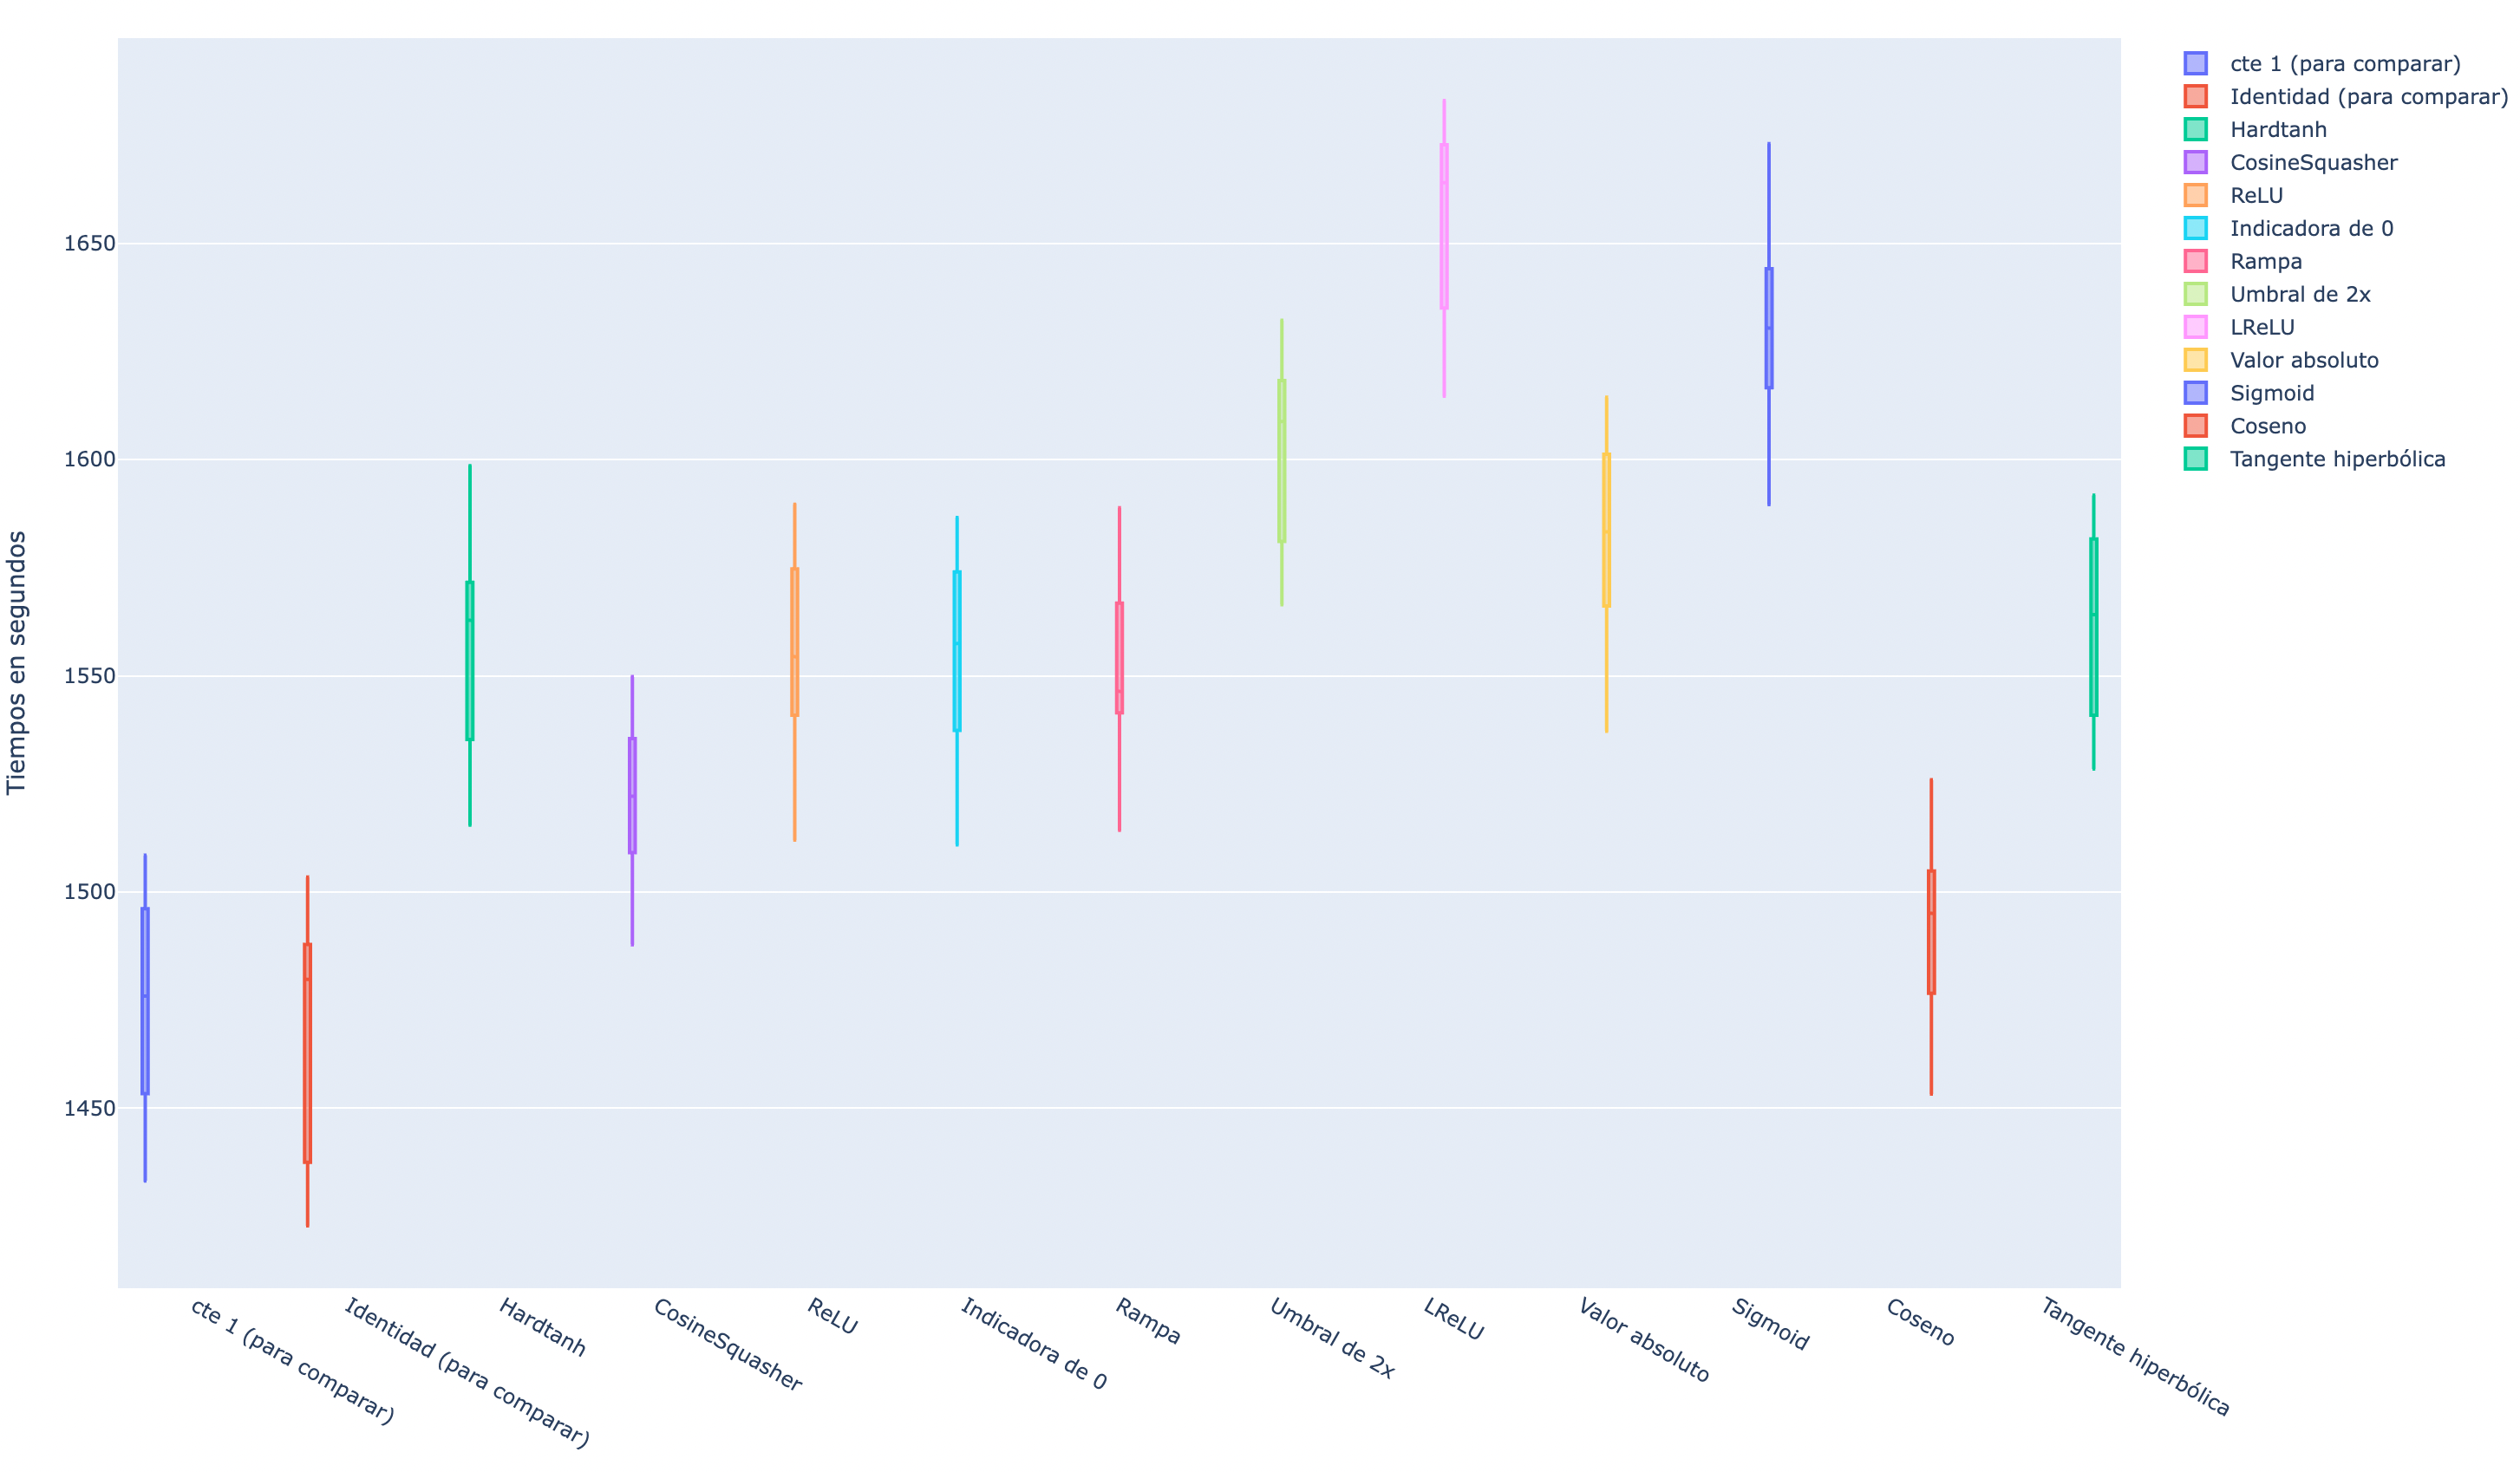
\includegraphics[width=\textwidth]{5-estudio-experimental/activation-function/boxplot-whiskers-activation-function.png}
     \caption{Gráfico de cajas y bigotes con los tiempo de las respectivas funciones}
     \label{img:boxplot-whiskers-activation-function}
\end{figure} 

Si volvemos a nuestro objetivo, que era encontrar el representante de 
menor costo entre las agrupaciones dispuestas en la tabla \ref{table:Clases-equivalencia-activation-function}. Concluimos que los mejores candidatos son: 

\begin{itemize}
    \item Para el \textit{grupo escalera}: No se ha rechazado la hipótesis nula, luego a priori no hay deferencia significativa y podemos seleccionar el candidato que queramos. 
    \item Para el \textit{grupo sigmoide}: La mejor opción ha sido \textit{Hard Hyperbolic Function} y  después en orden de mejor a peor: \textit{Cosine Squasher}, rampa, sigmoidea y tangente hiperbólica.
    \item Pare el \textit{grupo ReLU}: No se ha rechazado la hipótesis nula, así que no podemos decir nada. 
\end{itemize}

